\pdfoutput=1
\documentclass[%
% reprint,
%superscriptaddress,
%groupedaddress,
%unsortedaddress,
%runinaddress,
%frontmatterverbose, 
preprint,
%showpacs,preprintnumbers,
%nofootinbib,
%nobibnotes,
%bibnotes,
 amsmath,amssymb,
 aps,
%pra,
%prb,
%rmp,
%prstab,
%prstper,
%floatfix,
]{revtex4-1}

%usepackage[dvipdfmx]{graphicx}
%This(dvipdfmx) is added by Ichikata to inlude pdf figures in cygwin enviroment. You can delete.
\usepackage{graphicx}% Include figure files
\usepackage{dcolumn}% Align table columns on decimal point
\usepackage{bm}% bold math
\usepackage{color}
\usepackage{subfig}
\usepackage{multirow}
\usepackage{natbib}

%\usepackage{hyperref}% add hypertext capabilities
\usepackage[mathlines]{lineno}% Enable numbering of text and display math
%\usepackage{lineno}% Enable numbering of text and display math
%\linenumbers\relax % Commence numbering lines

%\usepackage[showframe,%Uncomment any one of the following lines to test 
%%scale=0.7, marginratio={1:1, 2:3}, ignoreall,% default settings
%%text={7in,10in},centering,
%%margin=1.5in,
%%total={6.5in,8.75in}, top=1.2in, left=0.9in, includefoot,
%%height=10in,a5paper,hmargin={3cm,0.8in},
%]{geometry}
\newcommand{\mtxtlbl}[1]{\text{{\scriptsize #1}}}

\begin{document}

\preprint{APS/123-QED}

\title{The $\nu$PRISM Detector}% Force line breaks with \\
%\thanks{A footnote to the article title}%


\collaboration{The $\nu$PRISM Collaboration}%\noaffiliation

\date{\today}% It is always \today, today,
             %  but any date may be explicitly specified

\begin{abstract}
Abstract here.
\begin{description}
\item[Usage]
Secondary publications and information retrieval purposes.
\item[PACS numbers]
May be entered using the \verb+\pacs{#1}+ command.
%\item[Structure]
%You may use the \texttt{description} environment to structure your abstract;
%use the optional argument of the \verb+\item+ command to give the category of each item. 
\end{description}
\end{abstract}

\pacs{Valid PACS appear here}% PACS, the Physics and Astronomy
                             % Classification Scheme.
%\keywords{Suggested keywords}%Use showkeys class option if keyword
                              %display desired
\maketitle

\tableofcontents
%\begin{linenumbers}%\relax % Commence numbering lines

\section{Introduction \label{sec:intro}}

%Neutrino oscillation experiments provide a window on to beyond the standard model physics of neutrino mass generation
% by measuring the properties of the neutrino mixing matrix and mass splittings.  The first observation of a 
%neutrino appearance signal by T2K~\cite{t2knue} has
% opened the door for the determination of the neutrino mass hierarchy and CP phase at current (T2K, NO$\nu$A) 
%and proposed (Hyper-K, LBNF, LBNO) long baseline accelerator experiments.  To make precision measurements of 
%oscillations parameters, including the CP violating phase, future experiments must achieve systematic uncertainties on 
%neutrino event rate predictions at the 2\% level or better.  In the current T2K $\nu_{e}$ appearance measurement, 
%the combined uncertainty on the neutrino flux and interaction modeling is 8\%, even with the constraint from 
%near detector data.  Significant improvements are needed to reach the level necessary for precision oscillation measurements.

Now that neutrino appearance has been observed by the T2K experiment~\cite{t2knue}, it is possible to determine the 
neutrino mass hierarchy and CP phase with current (T2K~\cite{Abe:2014tzr}, NO$\nu$A)  and proposed (Hyper-K~\cite{Abe:2011ts},
 LBNF, LBNO) long baseline 
accelerator experiments.  To make precision measurements of neutrino mixing parameters, including the CP violating phase, 
future experiments must achieve systematic uncertainties on neutrino event rate predictions at the 2\% level or better.  
The current T2K $\nu_{e}$ appearance measurement, the combined uncertainty on the neutrino flux and interaction modeling is 8.8\%.  
Significant improvements are therefore needed to reach the level necessary for precision oscillation measurements.

Substantial reduction to the overall systematic uncertainty is typically provided through the use of a near detector, 
which measures the initial rate of neutrino interactions prior to oscillation, however there are limitations to this technique 
as it is used currently.  First, the near detector measures abundant $\nu_\mu$ interactions to predict the oscillated $\nu_{e}$ 
event rate. In the T2K analysis, 3\% of the total uncertainty is based on theory calculations of the ratio of $\nu_{e}$ to $\nu_{\mu}$ 
cross sections; it is difficult to directly measure with comparable precision at the near detector as the $\nu_{e}$ component of 
the flux is significantly smaller by design. Second, uncertainties associated with the modeling of nuclear effects in neutrino 
interactions are significant in the T2K analysis; 7.5\% are uncertainties which do not cancel in the extrapolation. Third, 
reports of non-standard physics, such as sterile neutrinos, would modify the near detector event rate and affect the 
extrapolation; alternate explanations such as nuclear effects would also be relevant for the long baseline program.

In recent years, the incorporation of nuclear effects into the modeling of
neutrino interactions at the GeV scale has been a significant challenge.  The MiniBooNE 
"excess" of CCQE-like $\nu_{\mu}$ candidate events, particularly at large $Q^{2}$, 
has been interpreted as previously un-modeled nuclear effects which produce multi-nucleon final states with
no final state pions.  However, attempts to calculate these nuclear effects have provided disparate results, and there
is still no model that postdicts all of the experimental data.  Uncertainties associated with the
modeling of nuclear effects in neutrino interactions are expected to be a dominant systematic uncertainty
for future neutrino oscillation measurements.

Even if a model can correctly postdict observed event rates and kinematic distributions for a particular 
measurement an ambiguity often remains because the broad energy spectrum of neutrinos in neutrino beam presents
an under-constrained problem, {\it ie.} it is not possible to find a unique solution for the energy dependent 
neutrino interaction rate and final state particle kinematics that satisfies the data.  In one approach, the
under-constrained problem is addressed by combining constraints from different experiments with spectra peaked
at different energies.  However, the effectiveness of this approach can be limited due to systematic differences in 
measurements from multiple experiments.  A recent example is the seeming discrepancy in pion production spectra measured
by MiniBooNE and MINER$\nu$A which can be interpreted as unexplained energy dependence of the cross-section or merely
systematic effects unique to each experiment.

An experimental solution to these problems is to have a single 
experiment that over-constrains the problem by measuring the cross-section and final state particle kinematic distributions
for a range of spectra peaked at varying neutrino energies.  By making these measurements in a single experiment, the
relative systematic effects can be well understood.  If the neutrino flux can be predicted with enough accuracy, it 
may even be possible to extract the cross-section and final state particle kinematics over the energy region of interest
in a largely model-independent way (as one could do with a mono-energetic neutrino beam).

\subsection{The off-axis neutrino beam}
Current long base-line experiments such as T2K and NO$\nu$A use off-axis beams that take advantage of the two-body
decay kinematics of the charged pion to sample a narrow band beam.  Fig.~\ref{fig:off-axis} shows the spectra of $\nu_{\mu}$ 
neutrinos as a function of off-axis angle for the J-PARC neutrino beam.  An experiment that samples off-axis angles ranging
from 1 to 4 degrees observes neutrino spectra peaked between 400 MeV and 1000 MeV.  These off-axis spectra are relatively 
narrow in energy compared to on-axis fluxes (MiniBooNE, K2K) at similar peak energies.  Hence they can be used to provide
a stronger constraint on the energy dependence of the cross section and relationship between neutrino energy and 
final states.  

\begin{figure}
 \begin{center}
  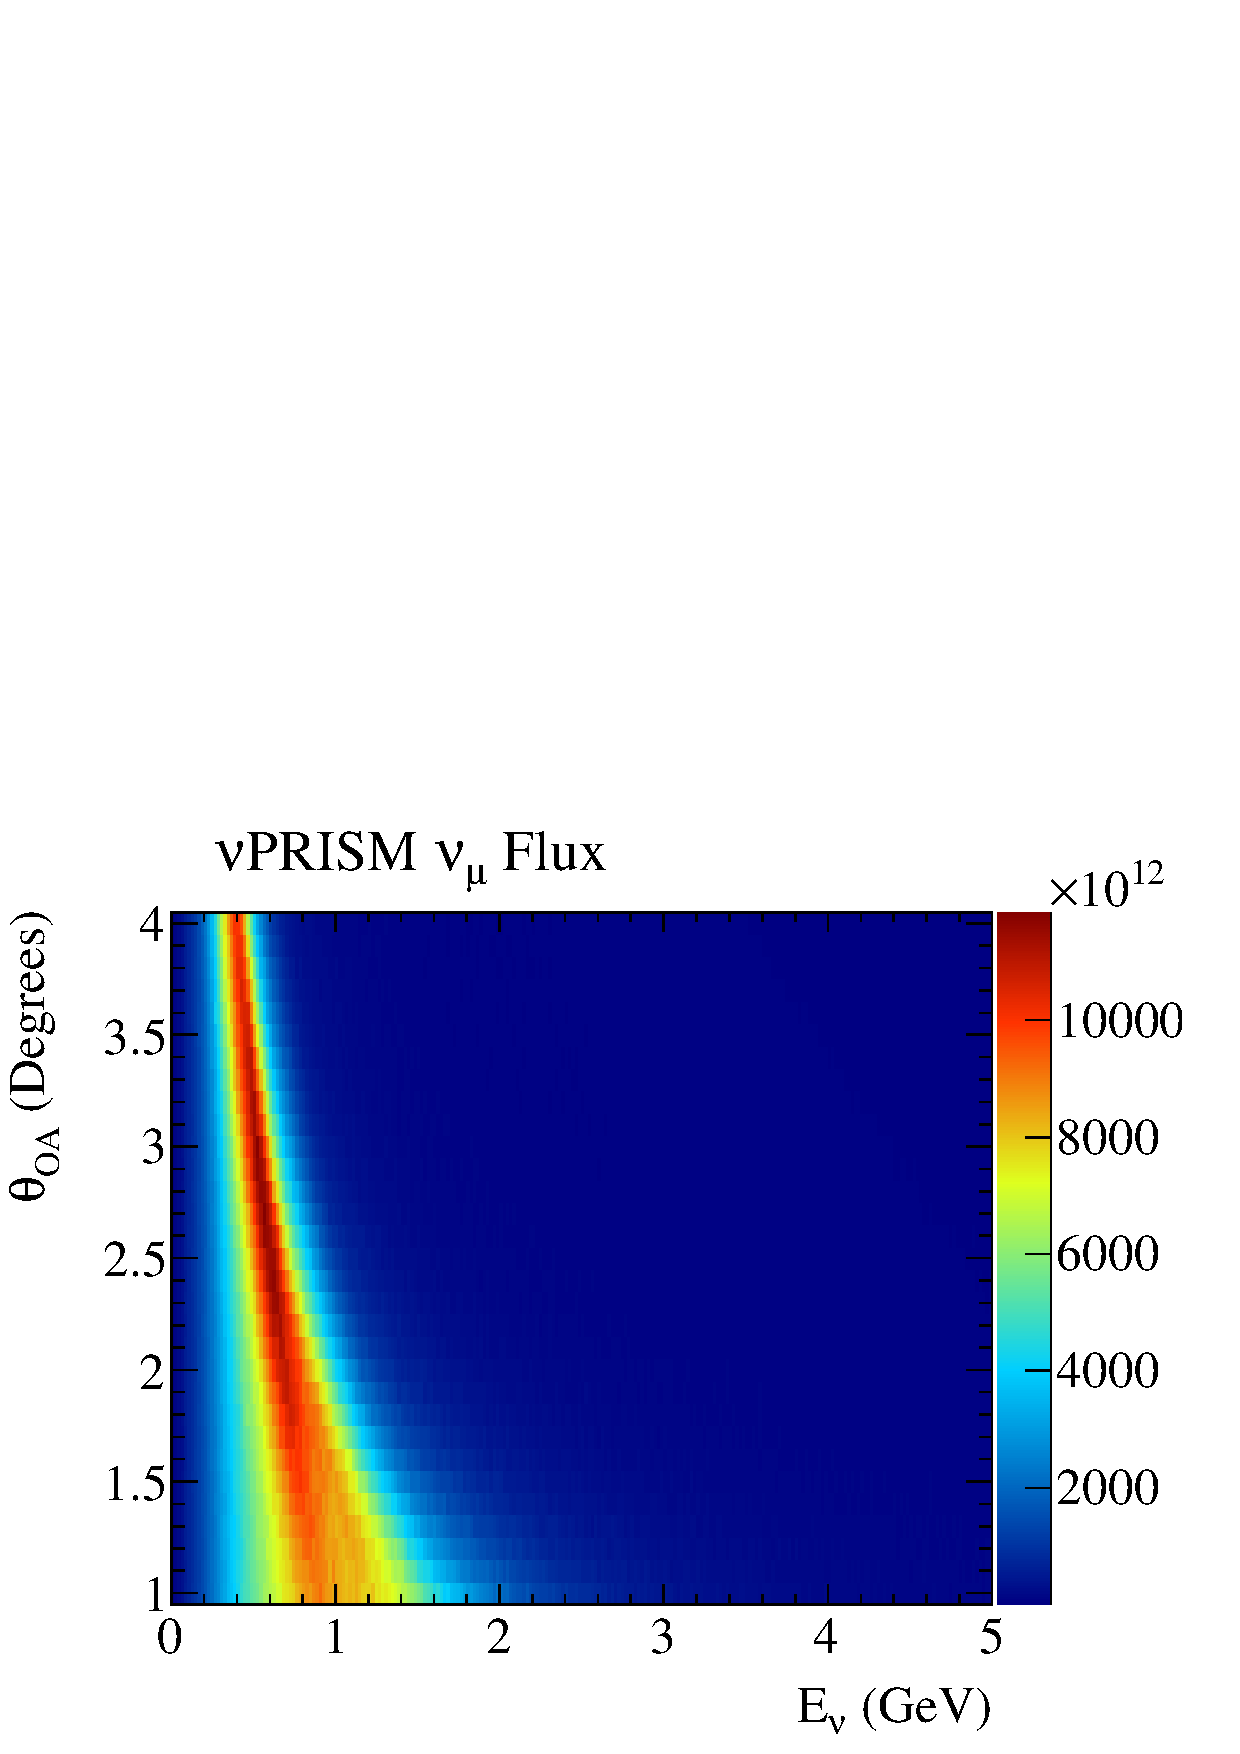
\includegraphics[width=0.45\textwidth]{figures/nuprism_oa_enu_numu.pdf}
  \caption{The $\nu_{\mu}$ flux spectra in the J-PARC neutrino beam for a range of off-axis angles.}
  \label{fig:off-axis}
  \end{center}
\end{figure}

A detector with a base line of $\sim1$~km and off-axis spectra may also be used to search for short-baseline neutrino oscillations
consistent with the LSND~\cite{Athanassopoulos:1996jb} or MiniBooNE~\cite{Aguilar-Arevalo:2013pmq} $\nu_{e}$ appearance anomalies.  
The observed excess in MiniBooNE may arise from 
oscillations associated with one or more sterile neutrinos, or more mundane mis-modeling of neutral current (NC) or charged current (CC) 
cross sections.  If sterile neutrinos are the cause of the excess, the energy dependence of the oscillations will lead to a 
unique pattern over the range of off-axis spectra that can be differentiated from mis-modelled interactions.

\subsection{The electron neutrino cross-section}
The neutrino oscillation channel used to probe for CP violation is $\nu_{\mu}(\bar{\nu}_{\mu})\rightarrow\nu_{e}(\bar{\nu}_{e})$.
While the beam observed by near detectors is $\sim99\%$ $\nu_{\mu}(\bar{\nu}_{\mu})$, the signal at the far detector
is $\nu_{e}(\bar{\nu}_{e})$.  Hence uncertainties in the relative cross-section of muon and electron neutrinos are also
critical.  Electron neutrinos of energy $~1$ GeV can be produced in the decays of muons, however, in conventional beams a
beam dump stops most muons before they decay.
In the absence of a stored muon beam, the study of the $\nu_{e}$ cross sections at $~1$ GeV is challenging.  Since the
$\nu_{e}$ component of the beam is only $~1\%$, a detector with a large fiducial mass and very pure particle identification 
capabilities is required.  Recent improvements in electron and $\pi^{0}$ separation in water Cherenkov detectors, and the capability 
of water Cherenkov detectors to scale to very large fiducial masses suggest that they can be used to measure the electron
neutrino cross section with unprecedented precision in a conventional neutrino beam.




\section{The $\nu$PRISM detector concept \label{sec:nuprism}}
The concept for the $\nu$PRISM detector is illustrated in Fig.~\ref{fig:nuprism_concept}.  It is a tall water-Cherenkov 
detector located 1-2~km from the neutrino source in J-PARC neutrino beam.  At 1~km, the detector is $\sim$50~m tall, covering
the off-axis angle range of 1-4 degrees. The base-line to the detector is set to at least 1~km to control event pile-up rates
and to reduce the line source effect of the pion beam.  A water-Cherenkov detector is chosen since measurements on H$_{2}$O are
most relevant for T2K and Hyper-K and the detector technology scales to large fiducial masses well.  The detector diameter is 
set to 10~m based on the need to contain forward going muons with momentum up to 1.5 GeV/c to probe the relevant phase space for
T2K and Hyper-K.  More details of the design considerations and construction techniques for $\nu$PRISM are given in 
Section~\ref{sec:nuprism_build}.

In $\nu$PRISM, a new off-axis angle, $\theta_{OA}$ observable is introduced.  This observable is estimated by using the reconstructed
vertex position for each event in $\nu$PRISM and calculating the angle between the average beam direction and the vector from the 
average neutrino production point to the reconstructed vertex.  A given $\theta_{OA}$ corresponds to a predicted neutrino spectrum,
and this additional information can be used to overconstrain the cross-section models or derive cross-sections in a model independent
way.

\begin{figure}
 \begin{center}
  \includegraphics[width=0.85\textwidth]{figures/nuprism_schematic.pdf}
  \caption{The $\nu$PRISM detector concept.}
  \label{fig:nuprism_concept}
  \end{center}
\end{figure}

\subsection{Measurments in $\nu$PRISM}
Charged current muon and electron neutrino interactions in $\nu$PRISM are identified by observing Cherenkov rings that
are consistent with penetrating or showering particles respectively.  Muon and electron candidates are further separated by the
presence of a delayed Michel electron from the muon decay.  Events with a single prompt muon or electron candidate ring are 
used for the oscillation candidate samples in T2K or Hyper-K oscillation measurements.  Table~\ref{tab:events} shows the number
and purity of these events in $\nu$PRISM at 1~km with a 1e21 proton-on-target exposure.

\begin{table}[tbh]
\caption{The $\nu$PRISM candidate event rates for single ring muon and electron like samples for 1e21 protons on target in
the J-PARC beam.}
\label{tab:events}
\begin{tabular}{l|cc|cc}
\hline
Off-axis Range & 1 Ring Muon Candidates & CC $\nu_{\mu}$ Purity & 1 Ring Electron Candidates & CC $\nu_{e}$ Purity \\
\hline
1$^{\circ}$-2$^{\circ}$ & 7.8e5 & 97.3\% & 5.4e3 & 32.5\%\\
2$^{\circ}$-3$^{\circ}$ & 4.3e5 & 97.7\% & 4.5e3 & 51.8\% \\
3$^{\circ}$-4$^{\circ}$ & 1.9e5 & 97.2\% & 2.9e3 & 65.0\% \\
\hline
\end{tabular}
\end{table}

The $\nu_{\mu}$ neutrino statistics and purity are high enough that the final state particle response can be derived for 
an almost arbitrary input spectrum using the information from the various off-axis spectra.  For example, the final state
muon momentum and scattering angle distributions for a nearly mono-energetic spectrum or an oscillated spectrum can 
be derived, as described in Section~\ref{sec:nuprism_numu}.

The $\nu_{e}$ statistics and purities in Table~\ref{tab:events} are derived using the same photo-coverage (40\%) and 
PMT size (20~inch) as Super-Kamiokande.  As was shown in the proposal for a 2~km water Cherenkov detector for T2K, smaller
PMTs with finer granularity can improve the performance, and that approach is being investigated for $\nu$PRISM. 
Regardless,
even with 1e21 protons on target and large PMTs, a measurement of the $\nu_{e}$ cross section with a 3\% statistical uncertainty
on the normalization is possible.  The $\nu_{e}$ candidate events will be used to measure the cross-section ratio relative to 
CC $\nu_{\mu}$ interactions and to search for short baseline $\nu_e$ appearance, as described in Section~\ref{sec:nuprism_numu}.

It is also possible to reconstruct events with two or more rings in $\nu$PRISM.  Events with a lepton candidate and additional 
charged particle ring can be used to measure the cross-section for single charged pion production in charged current interactions.
Events with two rings consistent with showering particles may be reconstructed as NC$\pi^{0}$ events, and events with a muon-like
particle that undergoes a hadronic scatter can be reconstructed as NC$\pi^{\pm}$ events.   For the neutral current events,
$\nu$PRISM provides a unique opportunity to directly measure the energy dependence of the cross-section in a single experiment.
These additional measurements with $\nu$PRISM are described in Section~\ref{sec:nuprism_other}.

\subsection{Flux modeling for $\nu$PRISM}
$\nu$PRISM takes advantage of the off-axis angle observable $\theta_{OA}$ to predict the underlying neutrino spectrum
for each interaction in $\nu$PRISM.  The predicted spectrum is based on the flux model.  For T2K the flux is predicted
based on a data-driven simulation of the neutrino beamline from the interaction of protons in the target to the decay of
hadrons and muons that produce neutrinos~\cite{Abe:2012av}.  The dominant uncertainties in the flux modeling arise from
modeling of hadronic interactions in the target, the magnetic horns and the decay region walls.  However, dedicated 
measurements from hadron production experiments such as NA61/SHINE are significantly reducing these uncertainties.  
These hadron production measurements include measurements of particle production multiplicities on replica targets.
By fully incorporating the replica target data, it is expected that experiments will be able to reduce uncertainties on the
flux prediction even lower than the $\sim10\%$ that has already been achieved by T2K and MiniBooNE~\cite{AguilarArevalo:2008yp}.  
With a precise 
flux prediction for $\nu$PRISM, the dependence of the neutrino spectra on $\theta_{OA}$ can be determined independently 
from $\nu$PRISM measurements, and that information can be incorporated in the derivation of neutrino cross-sections from the
$\nu$PRISM data. 

\section{Measurements with CC $\nu_{\mu}$ candidates \label{sec:nuprism_numu}}

% Need to somehow also talk about NC here too.

As discussed in the previous section, $\nu$PRISM can reconstruct large, pure samples of charged current
events with a muon candidate and no other particles above Cherenkov threshold.  For each event, the
off-axis angle $\theta_{OA}$ is reconstructed and this observable implies additional information about the
distribution of possible neutrino energies based on the prior flux model.  Data binned in $\theta_{OA}$ and the
usual muon observables of momentum (or kinetic energy) and scattering angle are used to constrain the
cross section model.  In the typical approach, the data may be unfolded to find the cross-section in the
true variable of neutrino energy, muon momentuma and muon scattering angle.  However, unfolding relies 
on regularization to deal with the ill-defined nature of the problem, and may not perform well when 
unfolding for $\theta_{OA}$ to the neutrino energy.

We take an alternative approach of using the off-axis neutrino spectra impinging on $\nu$PRISM as a set of basis
functions.  We then write a spectrum of interest as a linear combination of the off-axis spectra:
\begin{equation}
F_{\nu_{\mu}}(E_{\nu}) = \sum_{i} c_{i}\phi^{i}_{\nu_{\mu}}(E_{\nu}).
\end{equation}
Here $F_{\nu_{\mu}}(E_{\nu})$ is an arbitrary function of interest, $\phi^{i}_{\nu_{\mu}}(E_{\nu})$ is the predicted spectrum
in the $i^{th}$ off-axis angle bin and $c_{i}$ are simply coefficients.  The challenge is to find a set of $c_{i}$
that approximatly satisfy the equation while minimizing the statistical and systematic uncertainties that are propagated through the
linear combination.  Once the $c_{i}$ are found, we can write a similar equation for the observables:
\begin{equation}
N(p_{\mu},\theta_{\mu}|F_{\nu_{\mu}}(E_{\nu})) = \sum_{i} c_{i}N^{i}(p_{\mu},\theta_{\mu}).
\end{equation}
In this way, the final state particle multiplicities and kinematics can be measured for an given choice of 
of the input neutrino energy spectrum.  

The consequence of the nuPRISM flux combinations are that we can generate any neutrino flux shape within the kinematics specified by the detector position and beam line. Two immediate applications are evident: pseudo-monoenergetic neutrino beams for measurements of neutrino interactions on water, discussed in Section~\ref{sec:mono}, and the neutrino flux assuming a set of oscillation parameters, used  for long-baseline experiments such as T2K or Hyper-Kamiokande (Section~\ref{sec:oscd}) or atmospheric neutrino oscillation experiments.

\subsection{Pseudo-monoenergetic neutrino flux measurements}
\label{sec:mono}

% Neutrino vs. electron scattering.
%% Relevant variables of eA

While neutrinos are a unique probe of the axial structure of the nucleus, it has been challenging to use them. The canonical probe of nuclear structure is to scatter an electron of a known energy off a nuclear target. A comparison between the incident and recoil electron determines the energy transfer ($\omega$) and momentum transfer ($q^2$). Electron scattering experiments determine 

% Challenges of current measurements
%% CC1pi+ disagreement in deuterium data, CCQE axial form factor -> MEC?, NC/CC disagreements.
%% Flux averaged results, complicated by nuclear effects.

% What is possible with nuPRISM:
%% examples of mono energetic beams, ranges.
%% example eA plots?

% measurements of CCQE, CC1pi+
%% reference what has been done historically.
% nue/numu cross section ratio
% Unique measurements of NC processes.
%% Lack of information about NCpi+, NC1gamma. List of processes expected based on historic measurements **refs 1kton



\subsection{Oscillated }
\label{sec:oscd}


\section{Measurements with CC $\nu_{e}$ candidates \label{sec:nuprism_nue}}

\section{Other measurements in $\nu$PRISM \label{sec:nuprism_other}}


% Obsolete section?

\section{Detector design and construction considerations \label{sec:nuprism_build}}


\section{Conclusion \label{sec:summary}}


%\end{linenumbers}


%\begin{figure*}
%\includegraphics{fig_2}% Here is how to import EPS art
%\caption{\label{fig:wide}Use the figure* environment to get a wide
%figure that spans the page in \texttt{twocolumn} formatting.}
%\end{figure*}
%\begin{table*}
%\caption{\label{tab:table3}This is a wide table that spans the full page
%width in a two-column layout. It is formatted using the
%\texttt{table*} environment. It also demonstates the use of
%\textbackslash\texttt{multicolumn} in rows with entries that span
%more than one column.}
%\begin{ruledtabular}
%\begin{tabular}{ccccc}
% &\multicolumn{2}{c}{$D_{4h}^1$}&\multicolumn{2}{c}{$D_{4h}^5$}\\
% Ion&1st alternative&2nd alternative&lst alternative
%&2nd alternative\\ \hline
% K&$(2e)+(2f)$&$(4i)$ &$(2c)+(2d)$&$(4f)$ \\
% Mn&$(2g)$\footnote{The $z$ parameter of these positions is $z\sim\frac{1}{4}$.}
% &$(a)+(b)+(c)+(d)$&$(4e)$&$(2a)+(2b)$\\
% Cl&$(a)+(b)+(c)+(d)$&$(2g)$\footnotemark[1]
% &$(4e)^{\text{a}}$\\
% He&$(8r)^{\text{a}}$&$(4j)^{\text{a}}$&$(4g)^{\text{a}}$\\
% Ag& &$(4k)^{\text{a}}$& &$(4h)^{\text{a}}$\\
%\end{tabular}
%\end{ruledtabular}
%\end{table*}


\begin{acknowledgments}
Acknowledgments go here
\end{acknowledgments}

\bibliographystyle{unsrt}
\bibliography{NuPrismPaper}% Produces the bibliography via BibTeX.

\end{document}
